\documentclass[a4paper]{article}
\usepackage[spanish]{babel}
\usepackage[utf8]{inputenc}
\usepackage{charter}   % tipografia
\usepackage{graphicx}
\usepackage{wrapfig}
%\usepackage{makeidx}

%\usepackage{float}
%\usepackage{amsmath, amsthm, amssymb}
%\usepackage{amsfonts}
%\usepackage{sectsty}
%\usepackage{charter}
%\usepackage{wrapfig}
%\usepackage{listings}
%\lstset{language=C}


\usepackage{color} % para snipets de codigo coloreados
\usepackage{fancybox}  % para el sbox de los snipets de codigo

\definecolor{litegrey}{gray}{0.94}

% \newenvironment{sidebar}{%
% 	\begin{Sbox}\begin{minipage}{.85\textwidth}}%
% 	{\end{minipage}\end{Sbox}%
% 		\begin{center}\setlength{\fboxsep}{6pt}%
% 		\shadowbox{\TheSbox}\end{center}}
% \newenvironment{warning}{%
% 	\begin{Sbox}\begin{minipage}{.85\textwidth}\sffamily\lite\small\RaggedRight}%
% 	{\end{minipage}\end{Sbox}%
% 		\begin{center}\setlength{\fboxsep}{6pt}%
% 		\colorbox{litegrey}{\TheSbox}\end{center}}

\newenvironment{codesnippet}{%
	\begin{Sbox}\begin{minipage}{\textwidth}\sffamily\small}%
	{\end{minipage}\end{Sbox}%
		\begin{center}%
		\colorbox{litegrey}{\TheSbox}\end{center}}



\usepackage{fancyhdr}
\pagestyle{fancy}

%\renewcommand{\chaptermark}[1]{\markboth{#1}{}}
\renewcommand{\sectionmark}[1]{\markright{\thesection\ - #1}}

\fancyhf{}

\fancyhead[LO]{Sección \rightmark} % \thesection\ 
\fancyfoot[LO]{\small{Ituarte Joaquin, Lebrero Ignacio, Oller Luca}}
\fancyfoot[RO]{\thepage}
\renewcommand{\headrulewidth}{0.5pt}
\renewcommand{\footrulewidth}{0.5pt}
\setlength{\hoffset}{-0.8in}
\setlength{\textwidth}{16cm}
%\setlength{\hoffset}{-1.1cm}
%\setlength{\textwidth}{16cm}
\setlength{\headsep}{0.5cm}
\setlength{\textheight}{25cm}
\setlength{\voffset}{-0.7in}
\setlength{\headwidth}{\textwidth}
\setlength{\headheight}{13.1pt}

\renewcommand{\baselinestretch}{1.1}  % line spacing


% \setcounter{secnumdepth}{2}
\usepackage{underscore}
\usepackage{caratula}
\usepackage{url}
\usepackage{float}


% ******************************************************** %
%              TEMPLATE DE INFORME ORGA2 v0.1              %
% ******************************************************** %
% ******************************************************** %
%                                                          %
% ALGUNOS PAQUETES REQUERIDOS (EN UBUNTU):                 %
% ========================================
%                                                          %
% texlive-latex-base                                       %
% texlive-latex-recommended                                %
% texlive-fonts-recommended                                %
% texlive-latex-extra?                                     %
% texlive-lang-spanish (en ubuntu 13.10)                   %
% ******************************************************** %



\begin{document}


\thispagestyle{empty}
\materia{Organización del Computador II}
\submateria{Primer Cuatrimestre de 2015}
\titulo{Trabajo Práctico III}
\subtitulo{Tierra Pirata}
\grupo{Grupo Crash Bash/Ps1}
\integrante{Ituarte, Joaquin}{457/13}{joaquinituarte@gmail.com} % obligatorio 
\integrante{Lebrero, Ignacio}{751/13}{ignaciolebrero@gmail.com} % obligatorio 
\integrante{Oller, Luca}{667/13}{ollerrr@live.com} % obligatorio 

\maketitle
\newpage

\thispagestyle{empty}
\vfill

\thispagestyle{empty}
\vspace{3cm}
\tableofcontents
\newpage


\newpage

\section{Introducción}

En este informe explicaremos el desarrollo del código realizado para el trabajo práctico Tierra Pirata. El mismo consiste en realizar de forma simple un sistema operativo para comprender los fundamentos básicos de la misma área. 
\par La resolución de este trabajo es modulada, es decir, se resuelve dividiéndose en subproblemas, por lo que a medida que se realiza quedan algunas resoluciones definidas de forma genérica y/o solo su formato, las cuales se resolvieron luego en otro subproblema más avanzado.
\par La mayor parte del código generado por nosotros fue realizado en el lenguaje de programación C para simplificar la resolución y mejorar la claridad de las soluciones implementadas.
\par Es importante destacar además que a medida que se resolvieron los problemas, las soluciones fueron probadas para verificar su funcionamiento, pero debido a que no son relevantes a la resolución de los problemas en sí, no fueron incluidos en el código entregado.


\newpage
\section{Ejercicio I}

\subsection{Archivos Utilizados}

Con el fin de resolver el ejercicio, modificamos los siguientes archivos:

\begin{enumerate}

\item Gdt.c
\item kernel.asm

\end{enumerate}

\subsection{Explicación}
Comenzamos con crear nuestra Global Descriptor Table (de ahora en más, GDT). Los primeros descriptores de nuestra GDT están reservados por la cátedra, razón por la cual debemos comenzar a crear nuestros descriptores a partir de un offset de 8 descriptores (64 bytes) a partir de la dirección base de la GDT. A partir de este offset, definimos, en orden de aparición, algunos descriptores: ``código de nivel 0", ``código de nivel 3", ``datos de nivel 0", ``datos de nivel 3" $y$ ``datos de nivel 0" (este último usado para vídeo), con una diferencia de offset de 8 bytes entre descriptores.\\

Los descriptores tienen el siguiente formato:

\begin{enumerate}

\item Los primeros 4 descriptores definen su base como la dirección 0x00000000. El segmento de datos de video la define como 0x0000B8000.

\item El límite de los primeros 4 descriptores es de 127999 = 0x1F3FF (debemos direccionar 500MB en segmentos de 4kb $\rightarrow$ 500MB/4KB = 128000 $\rightarrow$ 127999 porque contamos el 0 como uno válido). El límite del descriptor de video es de 129024 = 0x1F800.

\item El tipo de segmento de los descriptores de código es de ejecución y lectura (tipo 10). El de los descriptores de datos (vídeo incluido) es de lectura y escritura (tipo 2).

\item Como ningún descriptor pertenece al sistema, el bit S lo seteamos en 1.


\item El tipo de descriptor de todos los descriptores es de código o datos (tipo 1, es decir, bit en 1).

\item Como nuestros segmentos son todos de 32 bits, el bit DB lo debemos setear en 1.

\item La granularidad (bit G) de todos los descriptores es de 1, dado que podemos usar hasta 4 GB.

\item Los bits DPL son seteados dependiendo del nivel de cada descriptor.

\item Seteamos el bit P de cada descriptor en 1 para indicar que el segmento está presente en la memoria RAM.

\end{enumerate}

\begin{figure}[ht!]
\centering
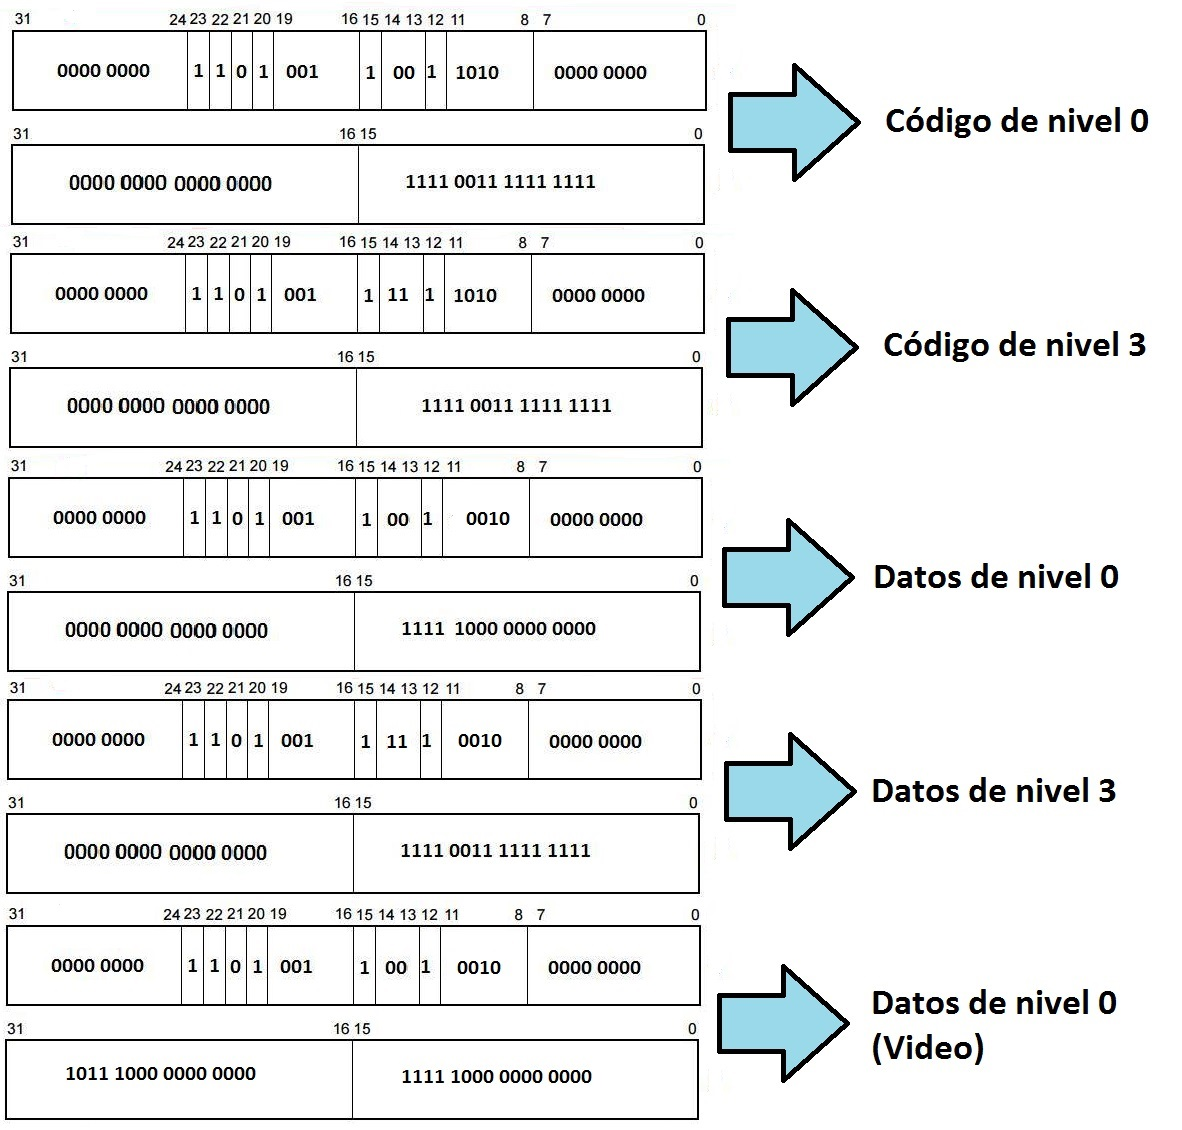
\includegraphics[width=100mm]{imagenes/GDTEJERCICIO1.jpg}
\caption{Entradas de la GDT}
\end{figure}

Para pasar a modo protegido (codeado en el archivo kernel.asm), debemos definir un entorno previo desactivando las interrupciones, cambiando el modo de video a 80 x 50 (debido a que la matriz de video es de 80 x 25 pixeles de 2 bytes cada uno), habilitando A20 usando la función provista por la cátedra, y cargando nuestra GDT ya definida.

Luego de haber preparado este entorno, pasamos a modo protegido seteando el bit PE del registro CR0 y hacemos un salto a una etiqueta en nuestro código llamada modoprotegido, en donde operamos sabiendo que ya estamos en este modo, llegando por medio de la instrucción jmp 0x40:modoprotegido, siendo 0x40 el offset del descriptor de segmento de código de nivel 0 de la GDT.


Ya en modo protegido, guardamos en los registros de segmento ds, es, gs y ss la dirección correspondiente al descriptor de segmentos de datos de nivel 0, y en el registro fs la dirección del descriptor correspondiente a los datos de video de nivel 0. También establecemos la base de la pila en la dirección 0x27000.

Luego de establecer la pila, procedimos a inicializar la pantalla. Para esto, hemos decidido implementar funciones en C, de forma tal que logremos imprimir una pantalla con fondo gris en la parte correspondiente al mapa de las tareas y con fondo negro en la parte inferior de la pantalla que corresponde al área donde imprimiremos información de cada jugador, representados cada uno con los colores rojo y azul.



\begin{figure}[ht!]
\centering
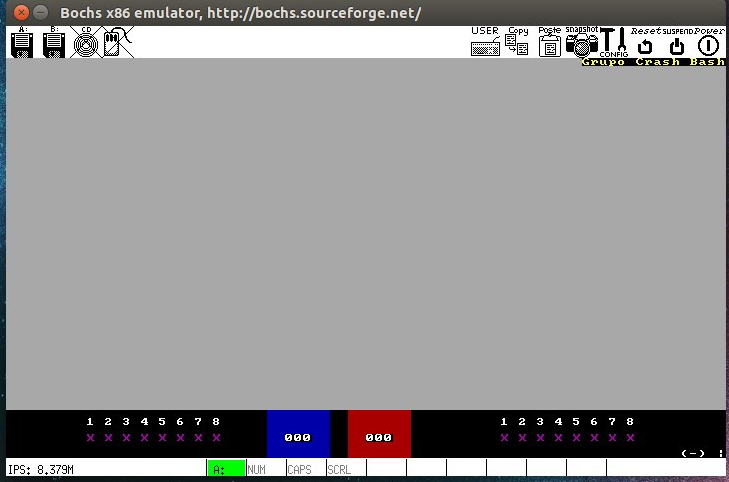
\includegraphics[width=100mm]{imagenes/imagenbochs.png}
\caption {Pantalla inicializada}
\end{figure}


\newpage

\section{Ejercicio II}
\subsection{Archivos Utilizados}

Con el fin de resolver el ejercicio, modificamos los siguientes archivos:

\begin{enumerate}

\item kernel.asm
\item idt.c
\item idt.h
\item isr.asm
\item isr.h

\end{enumerate}



\subsection{Explicación}
En este ejercicio debemos crear una IDT con 256 entradas. De estas entradas, nosotros debemos definir las primeras 20 entradas (contando desde 0) excepto las entradas 9 y 15. Las entradas no definidas quedan reservadas.\\
Las excepciones que nosotros definimos en una función de inicialización de la IDT son:
\begin{figure}[ht!]
\centering
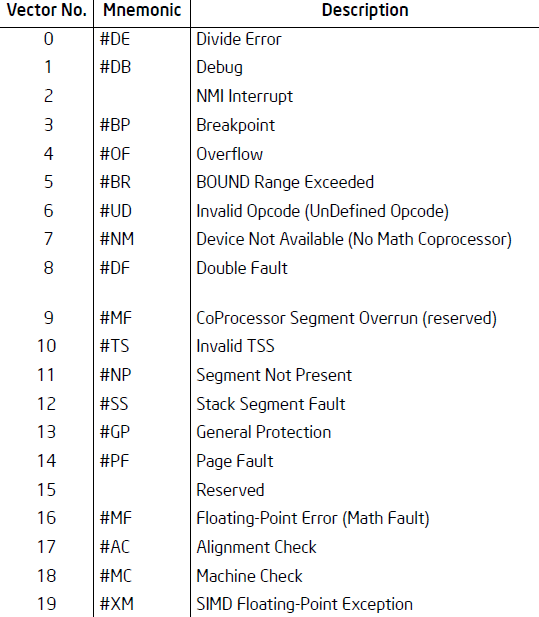
\includegraphics[width=100mm]{imagenes/Excepciones.png}
\caption {Tabla de excepciones.}
\end{figure}

A cada una de estas entradas las definimos en idt.c con el offset correspondiente a la rutina de la atención de la excepción correspondiente (las cuales se definirán luego en el archivo isr.asm), el selector de segmento correspondiente al segmento de código de nivel 0 (offset de GDT: 0x40) y los atributos seteados como: bit de presente (P) en 1, la prioridad es 0 y es de 32 bits (bit D en 1) (los atributos quedan expresados como 0x8E00).


\begin{figure}[ht!]
\centering
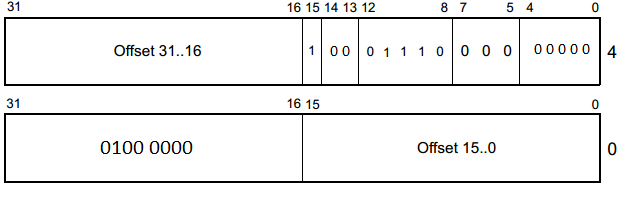
\includegraphics[width=100mm]{imagenes/IDTENTRY.png}
\caption {Entrada de una IDT, donde offset especifica la dirección de la rutina de atención.}
\end{figure}

Una vez realizado todo esto, en el archivo kernel.asm definimos la llamada a la inicialización (la llamada a la funcion recien explicada) y carga de la IDT y luego configuramos el controlador de interrupciones.\\


Luego en el kernel.asm, desactivamos el controlador de interrupciones del bios para comprobar el correcto funcionamiento de las funciones implementadas.


Por último para probar el correcto funcionamiento de las interrupciones intentamos dividir por cero y comprobar si iba a la interrupción correcta y le indicamos que realice un salto a sí mismo para tener un ciclo infinito dentro de la interrupción y así saber que funciona correctamente.













\newpage
\section{Ejercicio III}
\subsection{Archivos Utilizados}

Con el fin de resolver el ejercicio modificamos los siguientes archivos:

\begin{enumerate}
\item kernel.asm
\item screen.c
\item screen.h
\item mmu.c

\end{enumerate}


\subsection{Explicación}

Utilizando funciones implementadas en C, y aprovechando las funciones ya provistas por la cátedra, comenzamos limpiando la pantalla.

Luego implementamos la función mmu_inicializar_dir_kernel que inicializa el directorio de páginas del Kernel y las tablas de páginas del kernel (de 4 KB), mapenado con identity mapping las direcciones 0x00000000 - 0x003FFFFF en las direcciones 0x27000 (directorio de páginas del kernel) y 0x28000, 0x29000, 0x2A000 y 0x2B000 (tablas de páginas del kernel).

En el directorio de páginas definimos las Page Directory Entry(PDE) correspondientes a las 3 tablas de páginas que vamos a utilizar, con únicamente los bits de Lectura/Escritura y de Presente seteados en 1 y el resto en 0 (por ende, además, su nivel es de supervisor).

A cada una de las Page Table Entry (PTE) las definimos para que apunten entre las direcciónes 0x00000000 hasta la 0x003FFFFF, de a saltos de a 0x1000 por cada PTE definida. Los atributos de estas PTE van a ser todos iguales: nivel de supervisor, de escritura y que están presentes en la memoria. Además seteamos a los bit de accedidos y de modificado (dirty bit) en 0.

\begin{figure}[ht!]
\centering
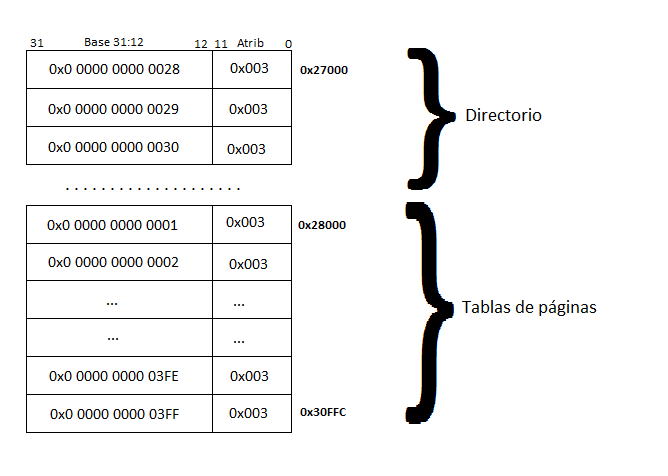
\includegraphics[width=100mm]{imagenes/DirectorioYTablas.png}
\caption {Representación en memoria del directorio y las tablas de páginas.}
\end{figure}



En esta parte del trabajo es donde también procedemos a activar paginación, simplemente definiendo cr3 con la dirección del directorio de páginas del kernel (0x27000) y seteando el bit más significativo de cr0 en 1.

Para finalizar el ejercicio, imprimimos en la esquina superior derecha de la pantalla $"$Grupo Crash Bash$"$ utilizando la función imprimir_texto_mp dada por la cátedra.


\newpage

\section{Ejercicio IV}
\subsection{Archivos Utilizados}

Con el fin de resolver el ejercicio, modificamos los siguientes archivos:

\begin{enumerate}

\item kernel.asm
\item mmu.c
\item mmu.h

\end{enumerate}


\subsection{Explicación}


Para esta parte del trabajo comenzamos realizando la inicialización de la mmu, que es simplemente definir que tenemos 768 páginas libres (1024 páginas totales menos 256 páginas usadas para el directorio del Kernel) y la dirección de la primera de ellas (0x100000). Estos datos se guardan en un objeto creado por nosotros mediante una estructura, con la cual mediante la función "mmu_gimme_gimme_page_wachin" se obtienen los mismos y los actualiza a medida que se llame a la función.

Luego continuamos por inicializar un directorio de páginas y tablas para una tarea (inicializar_dir_pirata). Para ésto pedimos una página con la función "mmu_gimme_gimme_page_wachin" que vamos a utilizar como el directorio de páginas del pirata. A todas las entradas de este directorio las definimos con el valor 0x02 para indicar que no tiene páginas presentes en memoria. Luego, definimos que el registro cr3 apunte a nuestro directorio de páginas. Luego, dependiendo de que jugador fue el que creo la tarea se le mapean las direcciones correspondientes a la posición inicial y los espacios adyacentes a él (con atributos 0x7 para página presente de nivel usuario lectura/escritura ) (De acá en adelante simplemente 0x3, 0x7 y 0x2 según corresponda).

Acto seguido movemos el código del pirata cuya implementación será explicada más adelante en este ejercicio. Finalmente se mapean como código de nivel 0 los directorios del kernel (con atributos 0x3 para página presente de lectura escritura de nivel supervisor).

A continuación definimos la función "mmu_mover_codigo_pirata", la cual se encarga de (dado un cr3, una posición física fuente y una destino) copiar el contenido de una página de memoria a otra y mapearlo al cr3 enviado. Para esto primero guardamos el cr3 de la tarea actual y mapeamos dos posiciones que estén sin uso en memoria (0x403000 y 0x404000) al fuente y destino como 0x7 y se procede a copiar el código posición por posición. Luego de haber realizado la copia simplemente se mapea al cr3 que se había enviado por parámetro la posición de destino a la posición virtual 0x400000 y se desmapean las posiciones sin uso previamente mapeadas.

Procedemos ahora a definir la función mmu_mapear_pagina, la cual recibe de parámetros la dirección virtual donde se ubica, la dirección física donde va a ser ubicada, el registro cr3 y los atributos que va a tener. Para esto obtenemos la dirección del directorio de páginas, la cual es cr3[31..12]:0x000. Luego obtenemos el offset del directorio, contenido en los bits 22-32 de la dirección virtual, y el offset de la tabla de páginas, contenida en los bits, 12-21, obteniendo así la entrada del directorio correspondiente a la tabla de páginas adecuada. Si esta entrada posee su bit de presente en 0, es decir que la tabla no está presente en memoria, pedimos con la función "mmu_gimme_gimme_page_wachin" una página nueva y redefinimos la entrada del directorio con la dirección de la página pedida y seteamos en 1 sus atributos de escritura y de presencia en la memoria. A la tabla de páginas obtenida, le seteamos en la entrada adecuada la dirección física con los atributos pasados como parámetros de la función. Finalmente utilizamos la función tlbflush para invalidar la caché de traducción de direcciones.

Para la realización de la función mmu_unmapear_pagina, la cual toma como parámetros una dirección virtual (que es la que se debe desmapear) y el registro cr3 (que contiene la dirección del directorio), usando la misma lógica para obtener la dirección de la entrada de la tabla de páginas que en la función para mapear, definimos el contenido de ésta con ceros, lo que hace que en sus atributos, el bit P indique que la página no está en memoria. Para finalizar la función, utilizamos la función tlbflush ya implementada por la cátedra.



\newpage

\section{Ejercicio V}
\subsection{Archivos Utilizados}

Con el fin de resolver el ejercicio, modificamos, además de kernel.asm los siguientes archivos:

\begin{enumerate}

\item idt.c
\item isr.h
\item isr.asm
\item sched.c

\end{enumerate}


\subsection{Explicación}

En este ejercicio comenzamos por definir las entradas en la IDT correspondiente a las interrupciones de reloj y de teclado. A éstas las definimos en las posiciones 32, 33 y 70 de la IDT respectivamente, definiéndoles a cada una el offset correspondiente a su rutina de atención de interrupción (definidas posteriormente en isr.asm), el selector de segmento correspondiente al segmento de código de nivel 0 (offset en GDT: 0x40) y los atributos seteados como: bit de presente (P) en 1, la prioridad es 0 y es de 32 bits (bit D en 1) (los atributos quedan expresados como 0x8E00). La interrupción de software 0x46 se diferencia de las anteriores solo en su dpl, el cual es 0x3 para que pueda ser llamada por tareas de nivel usuario, quedando los atributos expresados como 0xEE00.

A continuación debemos escribir la rutina de atención de la interrupción de reloj. Para esto, al comenzar la rutina indicamos que la interrupción fue atendida llamando a la función "fin_intr_pic1" provista por la cátedra. Luego realizamos el llamado a la función $"$game_tick$"$ y luego terminamos la interrupción. La función $"$game_tick $"$ realiza un llamado a la función "screen_actualizar_reloj_global" implementada por la cátedra. La funcionalidad total de "game tick" sera explicada mas adelante.

Para la rutina de atención de la interrupción del teclado, luego de llamar a la función "fin_intr_pic1", realizamos un código sencillo que imprima la tecla presionada en una posición arbitraria de la pantalla. Esta implementación fue reemplazada por la implementación para agregar una tarea nueva al jugador que oprima la tecla Shift (Right/Left dependiendo que jugador).

A éste ejercicio lo finalizamos definiendo una rutina simple de atención de la interrupción del sistema. Simplemente hacemos que la interrupción, luego de llamar a la función "fin_intr_pic1", escriba en el registro eax el valor 0x42.


\newpage

\section{Ejercicio VI}
\subsection{Archivos Utilizados}

Con el fin de resolver el ejercicio modificamos los siguientes archivos:

\begin{enumerate}

\item gdt.c
\item tss.c

\end{enumerate}


\subsection{Explicación}

\begin{description}

  \item[Ejercicio a, d y e:] Definimos en gdt.c, es decir en nuestra GDT, dos entradas nuevas correspondientes a la TSS inicial (entrada \#13) y la TSS idle (entrada \#14), ambas con las siguientes características: no están ocupadas (bit Busy en 0), es un descriptor de sistema (bit S en 0), con prioridad de nivel 0 (DPL = 0), presentes en memoria (P = 1) y con granularidad de 4 GB (G = 1). Las direcciones de memoria y los límites son definidos mediante la función en C ``tss_inicializar". Además definimos 16 entradas a tss libres (para lo cual debimos incrementar el tamaño de la gdt) con las caracteristicas:  type = 9, S = 0, dpl = 0, p = 0, g = 1;

\begin{figure}[ht!]
\centering
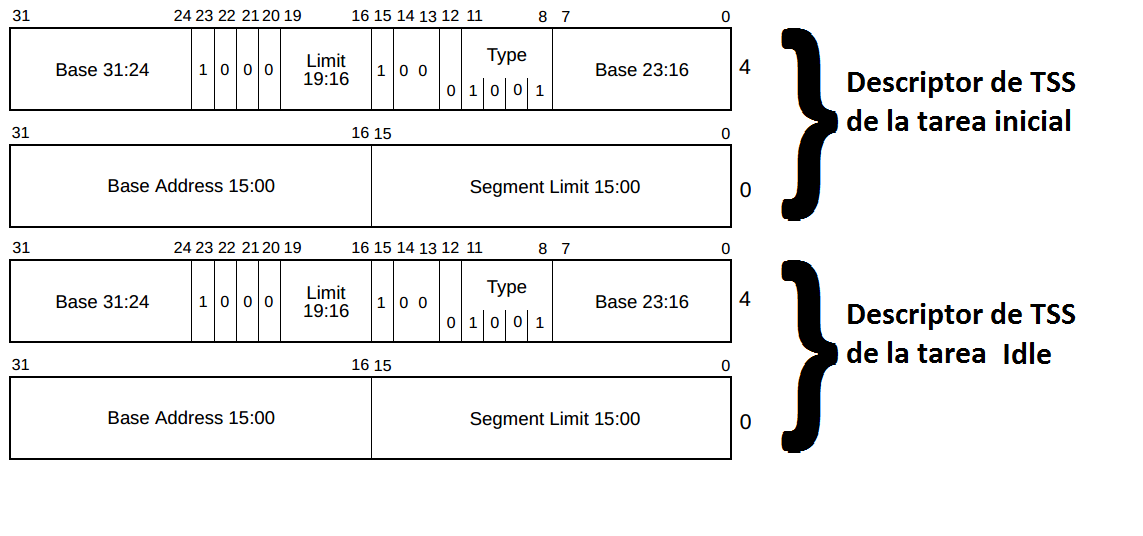
\includegraphics[width=100mm]{imagenes/Descriptortss.png}
\caption {Descriptor de TSS de las tareas inicial e Idle.}
\end{figure}
  
  \item[Ejercicio b:] Los datos de la entrada de la TSS de la tarea inicial son irrelevantes, motivo por el cual los definimos a todos en cero. A la entrada de la TSS de la tarea IDLE la completamos de la siguiente manera:

\begin{figure}[ht!]
\centering
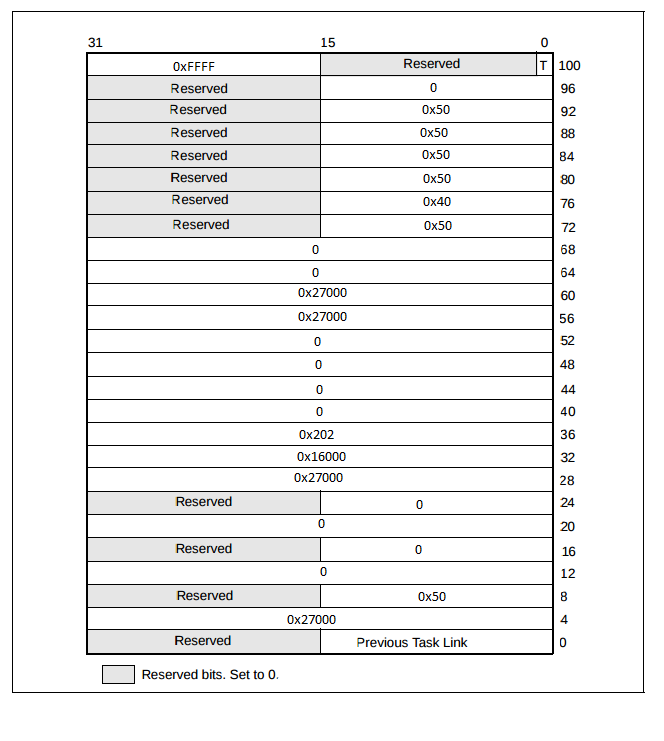
\includegraphics[width=100mm]{imagenes/tssincompleta.png}
\caption {TSS de la tarea idle}
\end{figure}
  
  \item[Ejercicio c:] La función que completa una TSS libre con los datos pasados por parámetro (el jugador y su posición correspondiente) la declaramos en tss.c y la llamamos inicializar_tarea.
  
  
  La TSS la completamos igual que en la idle a excepción de los siguientes registros:
  
  \begin{enumerate}
  \item eip : 0x400000.
  \item ss0    : 0x50. codigo de nivel 0
  \item ds     : 0x5B. segmento de datos de nivel 3
  \item esp0   : nueva pagina de memoria
  \item eflags : 0x202. interrupciones activadas
  \item ebp    : 0x401000
  \item esp    : 0x401000-0xC.
  \item gdt_posicion : obtiene un segmento disponible.
  \item cs, ss, ds, fs, gs : 0x4B. segmento de codigo de nivel 3
  
  \end{enumerate}
  
  Se coloca la base y el limite de dicho segmento, luego se apilan los parametros enviados a la pila de la tarea(recordar que los parametros tienen el formato (y $\ll$ 8 ) $\mathrel{|}$ x) y finalmente se retorna gdt_posicion shifteado 3 bits para no devolver los atributos de presente y de r/w.


\end{description}






\newpage

\section{Ejercicio VII}
\subsection{Archivos Utilizados}

Con el fin de resolver el ejercicio modificamos los siguientes archivos:

\begin{enumerate}

\item game.c
\item sched.c
\item gdt.c
\item tss.c
%\item 

\end{enumerate}




\subsection{Explicación}


\begin{description}

  \item[Ejercicio a] :\newline 
  Para la realización del scheduler, decidimos crear tres estructuras: ''tarea_scheduler'', ''sched_tareas'' y ''pirata''. 
  
  ''Tarea_scheduler'' es una estructura que representa a un jugador, contiene un arreglo de 8 ''piratas'', la cantidad de piratas que corren actualmente de este jugador y la posición del pirata que corre actualmente del mismo.
  
  ''sched_tareas'' representa al scheduler en si, contiene un arreglo de dos posiciones que contienen punteros a la tarea inicial del sistema y a la tarea Idle. Posee además dos objetos "tarea_scheduler" que representan a cada jugador, y guarda el turno del jugador actual. 
  
  ''pirata'' representa tan solo lo que es un pirata para el scheduler, una tarea, por lo que solo guarda el selector de la gdt al que corresponde y el id de la tarea.
  
%------------------------inicializacion-----------------------------%

Para la inicialización de este scheduler, lo que hacemos es crear un objeto de ''sched_tareas'' que va a tener definido para sus objetos de ''tarea_scheduler'' sus arreglos con id nulos, posiciones definidas como -1 y la cantidad de tareas establecidas en 0. Para sus otros atributos, se define en el arreglo de dos posiciones, en la primer posición un puntero a la tarea inicial, y en la segunda posición un puntero a la tarea Idle. Finalmente se define a la tarea actual del scheduler de forma arbitraria con un numero distinto a 0 o 1 para indicar que no es un dato válido.
  
Para dar de alta una tarea se llama a la función 'scheduler_agregar_tarea', la cual recibe el numero de jugador a la cual iniciar, la posición dentro del vector de tareas de ese jugador, el tipo de tarea(explorador o minero) y los parámetros para ser enviados a esa tarea al ejecutarse. Esta función simplemente revisa si no hay ningún jugador con tareas corriendo y de ser así asigna al jugador que lanzo la tarea el turno y luego llama a otra tarea que se encarga de llamar a 'inicializar_tarea', la cual inicializa una entrada libre de la tss (bit de presente en 0 en la gdt) y devuelve la posición de la entrada de ese segmento shifteada tres lugares a la izquierda. Luego se completan los campos del pirata creado. El id se genera como posición + (jugador * 8) de esta manera podremos más adelante dado un id, descomponerlo y saber a que jugador pertenece y en qué posición se encuentra dentro de los vectores correspondientes, esta definición la usamos para todas estructuras donde estén guardadas los piratas.

Para dar de baja a una tarea se llama a la función 'scheduler_matar_actual_tarea_pirata', esta decide cual es el jugador que cuya tarea corre actualmente y pasa a llamar a la función 'ejecutar_tarea', la cual dado un jugador (tarea_scheduler) setea el id del pirata actual en nulo y coloca un 0 en el bit de presente de su selector dentro de la gdt, de esta manera se los considerara libres a la hora de asignar una nueva tarea y no se los tendrá en cuenta cuando se quiera pasar a la próxima.
 
  
  \item[Ejercicio b] :\newline
  Para este punto usamos la función próxima_tarea, que dado un jugador (tarea_scheduler) revisa a partir de la posición del ultimo pirata que corría más uno, cual es el primer pirata con ID no nulo(ID_NULO = 17), y simplemente devuelve ese selector, de esta manera se modifica el estado de la estructura del jugador correspondiente para que cuando sea su turno nuevamente, éste continue con la próxima tarea. A diferencia del enunciado la función que decide que tarea corre a continuación será sched_tick, esta hace los chequeos de '¿Qué jugador corría previamente?', '¿El jugador que debería jugar ahora?, ¿Tiene tareas para correr?' y de esta manera chequea de quién será el turno. En caso de que se el turno de un jugador y este no tenga tareas para correr y el otro sí, se le concederá el turno al jugador con tareas. De no haber ningún pirata corriendo en el momento, se devolverá simplemente la tarea idle (ver Ejercicio 6)e) ).
  \item[Ejercicio c] :\newline
    Debido a decisiones de diseño este punto fue parcialmente explicado en el inciso b.
    La función 'proxima_tarea' devuelve el selector de la tarea que corre actualmente Esta función simplemente lo asigna y lo devuelve para que sea saltado.
  \item[Ejercicio d] :\newline
  
  Lo realizado en la syscall fue pushear todos los registros, luego pushear eax y ecx para pasarle como parámetros a la función game_syscall_manejar que ella se encarga de la lógica del juego, y luego que regresa de la función le sumamos 8 a la pila para alinearla (guardamos el eax de retorno en la pila, para que cuando se haga popad devolvamos el eax para los mineros) y hacemos un jmp far a la tarea idle ya que luego de que la tarea realiza su syscall pierde el turno.
  
  Game_syscall_manejar tiene 3 casos, el primero es si el pirata es un explorador, lo que hace es moverse, el segundo caso es si es un minero ya habiendo chequeado la posición (caso 3) se mueve y comienza a cavar y así sumar puntos.
  
  
      
  \item[Ejercicio e] :\newline
  
  En cada ciclo de reloj primero chequea si está activa la pantalla de debug, si está, no hace nada. Si no lo está, llama a la función sched_tick y carga cx con el task register y lo compara con lo obtenido en sched_tick, si son iguales no hace nada. Si no lo son, realiza un jmp far a la tarea devuelta en sched_tick.
  
  Sched_tick tiene dos casos principales, si es llamada y se estaba corriendo el jugador A o el B.
  
  En cualquiera de los casos, compara la cantidad de tareas del jugador si es mayor a 0, si lo es, asigna a scheduler.tarea_actual como jugador i y el selector correspondiente lo calcula a través de proxima tarea que toma como parámetro el scheduler.jugador_i.
  
  Si la cantidad de tareas del jugador llegase a ser 0, el procedimiento es primero fijarse si la cantidad de tareas del otro jugador es mayor a 0 y en ese caso coloca como selector a próxima_tarea tomando como parámetro el scheduler del otro jugador, en caso de no cumplirse esta condición se retorna la tarea idle.
  
  
  
  \item[Ejercicio f] :\newline
  
    La única modificación que debe realizarse es la de en cada rutina es que se haga un jmp a matar_pirata.
    
    Matar_pirata primero chequea si debug_activado está en 0, si lo está llama a game_pirata_explotó hecha en C que se encarga de desalojar la tarea.
    
    Si estaba habilitado el modo debuguer, primero coloca en 1 la variable pantalla_debug_activa y llama a la función screen_debuggear_tarea y luego llama a game_pirata_explotó.
    
    Antes de terminar pone a correr la tarea idle.
    
    Game_pirata_exploto llama a screen_matar_pirata con el pirata que estaba corriendo en ese momento, pone su id en NULL y llama a scheduler_matar_actual_tarea_pirata.
  
  
  \item[Ejercicio g] :

  Las rutinas que se ven modificadas son la del clock y la del teclado, en el caso del clock hace un chequeo si la variable debug_habilitado está en 1, salta al final.
  
  El teclado, por su parte lo que hace es, además de chequear si se tocan las teclas del juego. También compara la tecla Y y en caso de ser presionada si la variable debug_habilitado estaba en 1, entonces procede a deshabilitarlo.
  
  En el caso que estuviera deshabilitado, chequea si pantalla_debug_activa está en 1 si estaba, la deshabilita. 
  
  para armar la pantalla mandamos a una funcion en C los parametros por pila usando los que habian sido pusheados en al interrupcion, mientras que para los selectores de segmento recurrimos a funciones de la tss, los cuales dado un id devuelven el selector correspondiente(ss, ds, etc).

NOTAS:
1)Nuestra implementacion no redibuja la pantalla a su estado original luego de cerrar la pantalla debugger, esto se debe a que probamos varias posibles implementaciones pero no funcionaron:

-Intentamos crear un arreglo con la misma cantidad de posiciones que el mapa, guardar el estado previo y luego copiarlo, pero por algun motivo esto piso la direccion 0x10000 en donde se alojaba el codigo del pirataA, haciaendo que este no corriera.

-Otras implementaciones fueron una pedir paginas de memoria libre y otra mapear a direcciones que nunca usamos(por ejemplo la 0x406000) y copiar los uchar en ese lugar, pero ambas implementaciones no permitian que el juego siguiera al momento de redibujar la pantalla a su estado original, y luego de un tiempo se apagara bochs.
  
2)Para mostrar los registros crX intentamos usar las funciones provistar por la catedra rcrX() pero por algun motivo que desconocemos generaban errores, por este motivo se encuentran los campos vacios en el debugger
\end{description}


\end{document}
